\documentclass{article}
\usepackage{amsmath}
\usepackage{geometry}
\usepackage{graphicx}
\usepackage{epstopdf}
\setlength{\parindent}{0pt}
\usepackage{adjustbox}
\usepackage{caption}
\usepackage{float}
\usepackage{dsfont}
\usepackage{pdfpages}
\captionsetup[table]{labelformat=empty}
\geometry{hmargin=2.5cm,vmargin=2cm}
\DeclareMathOperator{\esp}{E}
\DeclareMathOperator{\cov}{cov}

\title{Valeurs manquantes, estimations manqu\'{e}es?}
\author{Nicolas Corneau-Tremblay}
\date{ao\^{u}t 2016}

\begin{document}
\maketitle

Ce document pr\'{e}sente (bri\`{e}vement) sous quelles conditions l'estimation de mod\`{e}les de r\'{e}gression \`{a} partir d'un \'{e}chantillon contenant des valeurs manquantes pose et ne pose pas  probl\`{e}me.

\section{Le cas g\'{e}n\'{e}ral}
Soit un mod\`{e}le de r\'{e}gression 

\[y=g(X)+u\]

o\`{u} $g(.)$ est une forme g\'{e}n\'{e}rale d\'{e}finissant la relation entre $y$ et $X$. L'esp\'{e}rance de $y$ conditionnelle \`{a} $X$ peut \^{e}tre \'{e}crite telle que

\[\esp(y|X)=g(X)+\esp(u|X)\]

Sous l'hypoth\`{e}se  que tous les \'{e}l\'{e}ments de $X$ sont orthogonaux au terme d'erreur, c'est-\`a-dire $\esp(u|X)=0$, l'estimation de

\[\esp(y|X)=\hat{g}(X)\]

peut \^{e}tre faite sans biais \`{a} l'aide d'un estimateur ad\'{equat}\footnote{D'autres hypoth\`{e}ses sont \'{e}galement n\'{e}cessaires pour effectuer cette estimation sans biais, mais leur importance est secondaire dans la pr\'{e}sente discussion.}. 
\\
\\
Soit \`{a} pr\'{e}sent un \'{e}chantillon contenant des valeurs manquantes pour certaines observations. Soit \'{e}galement $s$, une variable indicatrice prenant la valeur 0 si l'une des variables $\{y,X\}$ d'un individu est non-observ\'{e}e et 1 autrement. La s\'{e}lection des valeurs manquantes peut \^{e}tre due \`{a} un processus al\'{e}atoire affectant  soit $y$ ou $X$ (\textit{missing completely at random, MCAR}). Puisque ce processus survient de fa\c{c}on  al\'{e}atoire, il n'est li\'{e} \`{a} aucune caract\'{e}ristique particuli\`ere des individus. L'estimation de $g(.)$ peut donc \^{e}tre faite sans risque de biais, puisque $\esp(u|X)=0$ est toujours respect\'{e}e.
\\
\\
La s\'{e}lection peut aussi \^{e}tre due \`{a} un processus non-al\'{e}atoire qui est fonction des autres variables consid\'{e}r\'{e}es dans le mod\`{e}le de r\'{e}gression. Si la s\'{e}lection est fonction des variables ind\'{e}pendantes contenues dans $X$ (\textit{missing at random, MAR}), il est alors possible d'\'{e}crire la fonction suivante

\[s=h(X)\]

o\`{u} $s$, le fait pour un individu d'avoir une valeur manquante, suit une fonction $h(.)$ qui d\'{e}pend des variables ind\'{e}pendantes $X$. Dans ce cas,

\[\esp(u|X,s)=\esp(u|X,h(X))=\esp(u|X)\]

Puisque la variable $s$ d\'{e}pend uniquement des variables ind\'{e}pendantes $X$ \`{a} travers sa fonction $h(.)$, l'esp\'{e}rance de $u$ conditionnellement \`{a} $X$ n'est pas affect\'{e}e par $s$, le processus de s\'{e}lection. Ceci s'explique par le fait que lorsque $u$ est consid\'{e}r\'{e} en maintenant $X$ fixe, $s$ ne contient aucune variation, puisque lui m\^eme ne varie qu'en fonction de $X$. Le probl\`{e}me de r\'{e}gression demeure alors

\[\esp(y|X,s)=\esp(y|X)=g(X)+\esp(u|X)\]

et peut \^{e}tre estim\'{e} sans biais, toujours sous l'hypoth\`{e}se que $\esp(u|X)=0$.
\\
\\
Un probl\`{e}me dans l'estimation de la r\'{e}gression survient lorsque $s$ est fonction de $y$ (\textit{not missing at random, NMAR}), par exemple lorsque

\[s=h(y,X)\]

Dans ce cas alors

\[\esp(u|X,s)=\esp(u|X,h(y,X))\neq\esp(u|X)\]

puisque cette fois $s$ peut varier avec $y$ et ainsi faire varier $u$. Il est |`{a} noter que cela survient m\^{e}me lorsque $u$ est consid\'{e}r\'{e} en maintenant $X$ fixe et lorsque tous les \'{e}l\'{e}ments de $X$ sont orthogonaux \`{a} $u$. Le mod\`{e}le de r\'{e}gression souffre alors d'endog\'{e}n\'{e}it\'{e} et son estimation risque d'\^{e}tre biais\'{e}e, puisque

\[\esp(y|X,s)=g(X)+\esp(u|X,s)\]

o\`{u}

\[\esp(u|X,s)\neq0\]


\section{Le cas lin\'{e}aire}
Cette section investigue plus particuli\`{e}rement le probl\`{e}me de s\'{e}lection des variables manquantes pour le mod\`{e}le de r\'{e}gression lin\'{e}aire. Les r\'{e}sultats de la section pr\'{e}c\'{e}dente y sont d\'{e}velopp\'{e}s pour ce cas particulier. Soit un mod\`{e}le lin\'{e}aire

\begin{align}
\label{ml}
y=X\beta+u
\end{align}

o\`{u} $u\overset{i.i.d.}{\sim} N(0,\sigma^2)$ et o\`{u} l'hypoth\`{e}se $\esp(u|X)=0$ est respect\'{e}e. Le cas lin\'{e}aire o\`{u} $g(X)=X\beta$ est un cas particulier de la forme g\'{e}n\'{e}rale pr\'{e}sent\'{e}e dans la section pr\'{e}c\'{e}dente. Soit \'{e}galement $s=h(.)$ le processus de s\'{e}lection des valeurs manquantes. Par exemple, soit

\[s=\mathds{1}\{X<c\}\]

une fonction indicatrice prenant la valeur 1 si la valeur de $X$ est en dessous d'une constante $c$, et 0 si elle est \'{e}gale ou sup\'{e}rieure \`{a} $c$. Si $s=0$, alors l'individu poss\`{e}de une valeur manquante en $X$, ce qui est un cas de s\'{e}lection des valeurs manquantes sur les variables ind\'{e}pendantes (\textit{MAR}). Qu'advient-il alors du mod\`{e}le \`{a} estimer? Si l'on prend $\esp(y|X,s)$, l'\'{e}quation \eqref{ml} devient

\[\esp(y|X,s)=\esp(y|X,X<c)=X\beta+\esp(u|X,X<c)\]

Rappelons qu'un biais survient si $\esp(u|X,X<c)\neq0$. Cons\'{e}quemment au développement suivant 

\begin{align}
\esp(u|X,X<c) & = \esp[\esp(u|X=x)] \hspace{0.2cm} \forall \hspace{0.2cm}  X<c \hspace{0.2cm} \text{par la loi des esp\'{e}rances it\'{e}r\'{e}es} \nonumber \\
 & = \esp[0] \hspace{0.2cm} \text{puisque} \hspace{0.1cm} \esp(u|X=x)=0 \hspace{0.15cm} \text{sous l'hypoth\`{e}se} \hspace{0.1cm} \esp(u|X)=0 \nonumber \\
 & = 0 \nonumber 
\end{align}

il est possible de voir que le probl\`{e}me de biais ne se pose pas dans un mod\`{e}le lin\'{e}aire lorsque la s\'{e}lection des valeurs manquantes est faite sur les variables ind\'{e}pendantes.
\\
\\
Soit \`{a} pr\'{e}sent

\[s=\mathds{1}\{y<c\}\]

Dans ce cas, la s\'{e}lection s'effectue sur la variable d\'{e}pendante (\textit{NMAR}). L'\'{e}quation \eqref{ml} devient cette fois

\[\esp(y|X,s)=\esp(y|X,y<c)=X\beta+\esp(u|X,y<c)\]

Encore une fois, un biais survient si $\esp(u|X,y<c)\neq0$. Dans ce cas

\begin{align}
\esp(u|X,y<c) & = \esp(u|X,X\beta+u<c) \nonumber \\
 & = \esp(u|X\beta+u<c) \nonumber \\
 & = \esp(u|u<c-X\beta) \nonumber \\
 & = \sigma\esp\left(\left. \frac{u}{\sigma}\  \right\rvert \frac{u}{\sigma}< \frac{c-X\beta}{\sigma} \right)  \nonumber \\
  & = \sigma\left[ \frac{\phi(c-X\beta)}{\Phi(c-X\beta)}\ \right] \hspace{0.1cm}  \text{sous l'hypoth\`{e}se} \hspace{0.1cm} u\overset{i.i.d.}{\sim} N(0,\sigma^2) \nonumber
\end{align}

Alors $\esp(y|X,s)$ devient

\begin{align}
\esp(y|X,s) & =X\beta+\esp(u|X,y<c) \nonumber \\
& = X\beta+\sigma\left[ \frac{\phi(c-X\beta)}{\Phi(c-X\beta)}\ \right] \nonumber
\end{align}

o\`{u} $\phi(.)$ et $\Phi(.)$ sont respectivement la fonction de densit\'{e} et la fonction de re
\'{e}partition de la loi normale centr\'{e}e r\'{e}duite. Il est possible de voir que $\esp(u|X,y<c)\neq0$, et donc que l'estimation d'un mod\`{e}le lin\'{e}aire qui ne prend pas un compte la s\'{e}lection sur $y$ m\`{e}ne \`{a} des param\`{e}tres biais\'{e}s.




\section{Simulation}
Il est possible d'explorer ces preuves th\'{e}oriques \`{a} l'aide d'une simulation. 

\subsection{R\'{e}gressions lin\'{e}aires simples}
Soit le mod\`{e}le de r\'{e}gression

\begin{equation}
\label{modele}
y=\alpha+\beta_1exposition+\beta_2x+\beta_3interaction+u
\end{equation}

o\`{u}

\[exposition\sim N(0,1)\]
\[x\sim N(0,1)\]
\[interaction=exposition*x\]
\[u \overset{i.i.d.}{\sim} N(0,1)\]
et
\[\alpha=\beta_1=\beta_2=\beta_3=1\]

Les variables $exposition$, $x$, $interaction$ et $y$ ont \'{e}t\'{e} cr\'{e}\'{e}es par simulation\footnote{L'ensemble du code et de l'output \textit{Stata} utilis\'{e} dans cette section et la suivante est disponible en Appendix du pr\'{e}sent document.}. En estimant le mod\`{e}le de r\'{e}gression pr\'{e}sent\'{e} en \eqref{modele} \`{a} partir de donn\'{e}es simul\'{e}es, Les r\'{e}sultats suivant sont obtenus

\def\onepc{$^{\ast\ast}$} \def\fivepc{$^{\ast}$}
\def\tenpc{$^{\dag}$}
\def\legend{\multicolumn{4}{l}{\footnotesize{Significance levels
:\hspace{1em} $\dag$ : 10\% \hspace{1em}
$\ast$ : 5\% \hspace{1em} $\ast\ast$ : 1\% \normalsize}}}
\begin{table}[H]\centering
 \caption{R\'{e}gression : mod\`{e}le de base
\label{tabresult regress}}
\begin{tabular}{l r @{} l c }\hline\hline 
\multicolumn{1}{c}
{\textbf{Variable}}
 & \multicolumn{2}{c}{\textbf{Coefficient}}  & \textbf{(Std. Err.)} \\ \hline
expo  &  1.019&\onepc  & (0.033)\\
x  &  1.015&\onepc  & (0.032)\\
inter  &  1.024&\onepc  & (0.033)\\
Intercept  &  0.959&\onepc  & (0.032)\\
\hline
\multicolumn{4}{c}{}\\
\hline N & \multicolumn{3}{c}{1000}\\
R$^{2}$ & \multicolumn{3}{c}{0.738}\\
F $ _{(3,996)}$ & \multicolumn{3}{c}{936.143}\\
\hline
\legend
\end{tabular}
\end{table}

Les r\'{e}sultats sont coh\'{e}rents, puisque chaque param\`{e}tre est relativement pr\`{e}s de sa vraie valeur.
\\
\\
Le premier type de valeur manquante abord\'{e} pr\'{e}c\'{e}dement est celui d\^{u} \`{a} un processus al\'{e}atoire. Ainsi, en retirant de fa\c{c}on al\'{e}atoire le $1/4$ de l'\'{e}chantillon simul\'{e}, l'estimation des param\`{e}tres devient

\def\onepc{$^{\ast\ast}$} \def\fivepc{$^{\ast}$}
\def\tenpc{$^{\dag}$}
\def\legend{\multicolumn{4}{l}{\footnotesize{Significance levels
:\hspace{1em} $\dag$ : 10\% \hspace{1em}
$\ast$ : 5\% \hspace{1em} $\ast\ast$ : 1\% \normalsize}}}
\begin{table}[H]\centering
 \caption{R\'{e}gression : s\'{e}lection al\'{e}atoire (MCAR)
\label{tabresult regress}}
\begin{tabular}{l r @{} l c }\hline\hline 
\multicolumn{1}{c}
{\textbf{Variable}}
 & \multicolumn{2}{c}{\textbf{Coefficient}}  & \textbf{(Std. Err.)} \\ \hline
expo  &  1.059&\onepc  & (0.037)\\
x  &  1.041&\onepc  & (0.038)\\
inter  &  1.031&\onepc  & (0.040)\\
Intercept  &  0.971&\onepc  & (0.036)\\
\hline
\multicolumn{4}{c}{}\\
\hline N & \multicolumn{3}{c}{750}\\
R$^{2}$ & \multicolumn{3}{c}{0.739}\\
F $ _{(3,746)}$ & \multicolumn{3}{c}{703.928}\\
\hline
\legend
\end{tabular}
\end{table}

Comme anticip\'{e}, les r\'{e}sultats sont encore une fois coh\'{e}rents.
\\
\\
Le second type de valeurs manquantes est lorsqu'une s\'{e}lection sur les variables ind\'{e}pendantes survient. Dans le cas pr\'{e}sent, le $1/4$ de l'\'{e}chantillon ayant les plus grandes valeurs pour $x$ a \'{e}t\'{e} retir\'{e}. Les r\'{e}sultats sont

\def\onepc{$^{\ast\ast}$} \def\fivepc{$^{\ast}$}
\def\tenpc{$^{\dag}$}
\def\legend{\multicolumn{4}{l}{\footnotesize{Significance levels
:\hspace{1em} $\dag$ : 10\% \hspace{1em}
$\ast$ : 5\% \hspace{1em} $\ast\ast$ : 1\% \normalsize}}}
\begin{table}[H]\centering
 \caption{R\'{e}gression : s\'{e}lection sur x (MAR)
\label{tabresult regress}}
\begin{tabular}{l r @{} l c }\hline\hline 
\multicolumn{1}{c}
{\textbf{Variable}}
 & \multicolumn{2}{c}{\textbf{Coefficient}}  & \textbf{(Std. Err.)} \\ \hline
expo  &  1.019&\onepc  & (0.042)\\
x  &  0.972&\onepc  & (0.051)\\
inter  &  1.028&\onepc  & (0.053)\\
Intercept  &  0.932&\onepc  & (0.042)\\
\hline
\multicolumn{4}{c}{}\\
\hline N & \multicolumn{3}{c}{750}\\
R$^{2}$ & \multicolumn{3}{c}{0.576}\\
F $ _{(3,746)}$ & \multicolumn{3}{c}{337.975}\\
\hline
\legend
\end{tabular}
\end{table}

Malgr\'{e} une s\'{e}lection forte sur une variable ind\'{e}pendante et la perte de beaucoup d'observations, les estimations ne semblent pas \^{e}tre affect\'{e}es. Il est \`{a} noter que ce r\'{e}sultat est v\'{e}rifi\'{e} m\^{e}me si la variable $x$ est corr\'{e}l\'{e}e \`{a} la variable $exposition$.
\\
\\
Enfin, le dernier type de valeur manquante est celui o\`{u} une s\'{e}lection est faite sur la variable d\'{e}pendante. Dans le cas pr\'{e}sent, le $1/4$ de l'\'{e}chantillon ayant les plus grandes valeurs pour $y$ a \'{e}t\'{e} retir\'{e}. Les r\'{e}sultats obtenus sont les suivants

\def\onepc{$^{\ast\ast}$} \def\fivepc{$^{\ast}$}
\def\tenpc{$^{\dag}$}
\def\legend{\multicolumn{4}{l}{\footnotesize{Significance levels
:\hspace{1em} $\dag$ : 10\% \hspace{1em}
$\ast$ : 5\% \hspace{1em} $\ast\ast$ : 1\% \normalsize}}}
\begin{table}[H]\centering
 \caption{R\'{e}gression : s\'{e}lection sur y (NMAR)
\label{tabresult regress}}
\begin{tabular}{l r @{} l c }\hline\hline 
\multicolumn{1}{c}
{\textbf{Variable}}
 & \multicolumn{2}{c}{\textbf{Coefficient}}  & \textbf{(Std. Err.)} \\ \hline
expo  &  0.746&\onepc  & (0.040)\\
x  &  0.731&\onepc  & (0.041)\\
inter  &  0.834&\onepc  & (0.041)\\
Intercept  &  0.589&\onepc  & (0.038)\\
\hline
\multicolumn{4}{c}{}\\
\hline N & \multicolumn{3}{c}{750}\\
R$^{2}$ & \multicolumn{3}{c}{0.442}\\
F $ _{(3,746)}$ & \multicolumn{3}{c}{196.821}\\
\hline
\legend
\end{tabular}
\end{table}

Dans ce dernier exemple, on vient bien que la s\'{e}lection non-al\'{e}atoire sur $y$ cause de lourds probl\`{e}mes de biais. Les param\`{e}tres d\'{e}vient fortement de leur vraie valeur. Ces r\'{e}sultats sont coh\'{e}rents avec les pr\'{e}sentations th\'{e}oriques faites dans les sections pr\'{e}c\'{e}dentes.


\subsection{Monte Carlo}
Soit le m\^{e}me mod\`{e}le de r\'{e}gression qu'en \eqref{modele}

\[y=\alpha+\beta_1exposition+\beta_2x+\beta_3interaction+u\]


Cette sous-section pr\'{e}sente les densit\'{e}s estim\'{e}es des param\`{e}tres de r\'{e}gression pour $exposition$ et $interaction$ pour 1000 it\'{e}rations. Elles ont \'{e}t\'{e} estim\'{e}es pour chacun des types de s\'{e}lections de la sous-section pr\'{e}c\'{e}dente.

\begin{figure}[H]
\centering
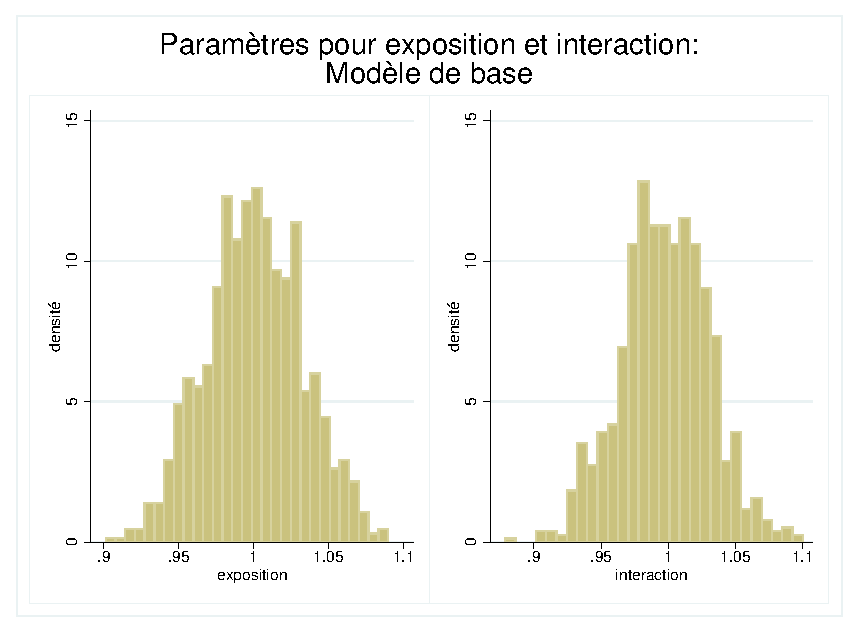
\includegraphics[scale=1]{model.eps}
\end{figure}

\begin{figure}[H]
\centering
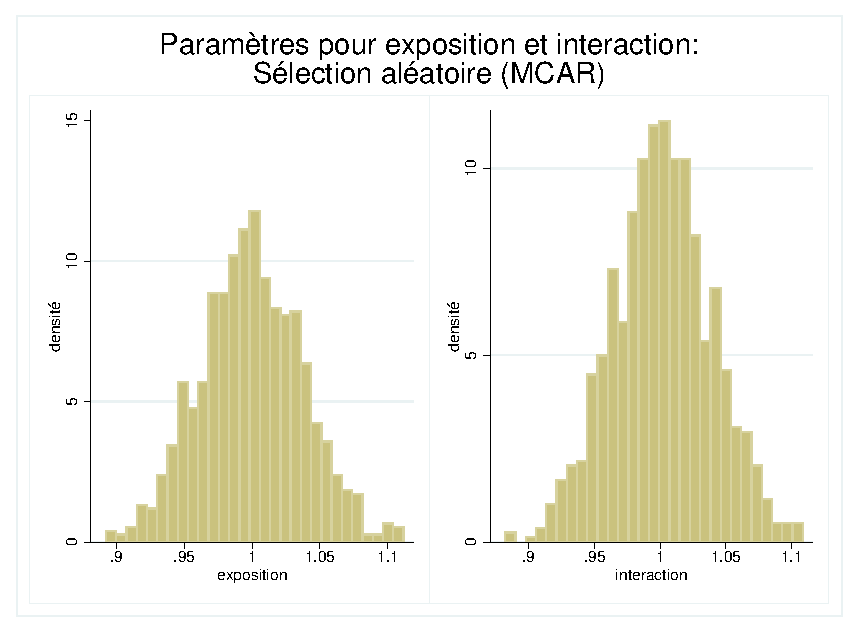
\includegraphics[scale=1]{random.eps}
\end{figure}

\begin{figure}[H]
\centering
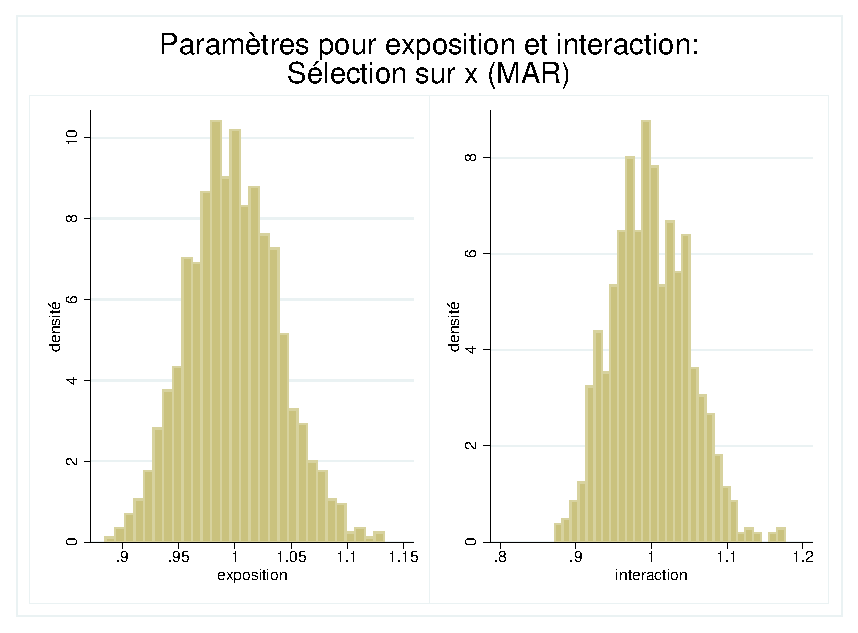
\includegraphics[scale=1]{selectx.eps}
\end{figure}

\begin{figure}[H]
\centering
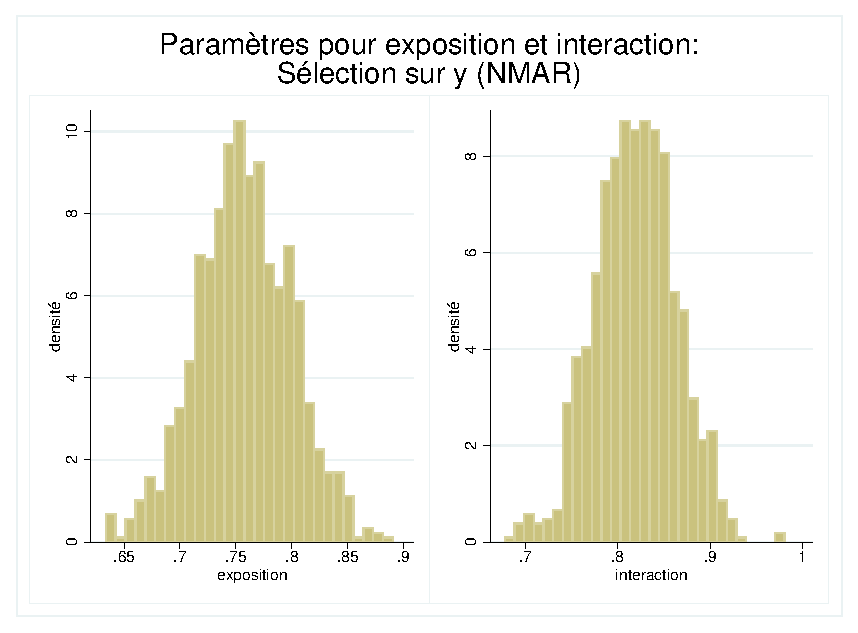
\includegraphics[scale=1]{selecty.eps}
\end{figure}

Cet exemple apporte une autre preuve que seul le processus de s\'{e}lection sur $y$ cause des probl\`{e}mes syst\'{e}matiques de biais. En effet, comme le montrent les histogrammes, seul ce processus fait immanquablement d\'{e}vier les param\`{e}tres estim\'{e}s de leur vraie valeur.


\appendix

\newpage

\section{Variable omise : le cas lin\'{e}aire}
Un probl\`{e}me similaire (mais distinct) \`{a} celui des valeurs manquantes est celui des variables omises. Le cas lin\'{e}aire est abord\'{e} dans cette section, notamment les conditions n\'{e}cessaires pour que l'omission d'une variable cause un probl\`{e}me de biais d'estimation dans les  param\`{e}tres.
\\
\\
Soit, par exemple, le mod\`{e}le lin\'{e}aire 

\begin{equation}
\label{mco}
y=\alpha+\beta_1X+\beta_2s+u
\end{equation}

o\`{u} cette fois $s$ n'est plus le processus de s\'{e}lection des valeurs manquantes mais une simple variable. L'estimation de l'\'{e}quation en \eqref{mco} peut \^{e}tre faite par moindres carr\'{e}s ordinaires, menant aux \'{e}quations 

\[\hat{\beta}_1=\frac{\sum_{i=1}^N(X_i-\bar{X})y_i}{\sum_{i=1}^N(X_i-\bar{X})^2}\]
\[\hat{\beta}_2=\frac{\sum_{i=1}^N(s_i-\bar{s})y_i}{\sum_{i=1}^N(s_i-\bar{s})^2}\]
\[\hat{\alpha}=\bar{y}-(\hat{\beta}_1\bar{X}+\hat{\beta}_2\bar{s})\]

Sous l'hypoth\`{e}se que les variables $\{X,s\}$ sont exog\`{e}nes, l'estimation se fait sans biais. 
\\
Cependant, si au lieu de l'\'{e}quation \eqref{mco}, l'\'{e}quation

\begin{equation}
\label{biais}
y=\alpha+\beta_1X+\tilde{u}
\end{equation}

est estim\'{e}e, o\`{u} $\tilde{u}=\beta_2s+u$, alors l'omission de la variable $s$ dans l'estimation peut engendrer un biais dans les autres param\`{e}tres. Pour bien voir cela, il est possible d'\'{e}crire 

\begin{align}
 \hat{\beta}_1 & =\frac{\sum_{i=1}^N(X_i-\bar{X})y_i}{\sum_{i=1}^N(X_i-\bar{X})^2} \nonumber \\
 & = \frac{\sum_{i=1}^N(X_i-\bar{X})(\alpha+\beta_1X_i+\beta_2s_i+u_i)}{\sum_{i=1}^N(X_i-\bar{X})^2} \nonumber \\
 & = \beta_1+ \beta_2\frac{\sum_{i=1}^N(X_i-\bar{X})s_i}{\sum_{i=1}^N(X_i-\bar{X})^2} + \frac{\sum_{i=1}^N(X_i-\bar{X})u_i}{\sum_{i=1}^N(X_i-\bar{X})^2} \nonumber
\end{align}

Sous l'hypoth\`{e}se que $\sum_{i=1}^N(X_i-\bar{X})u_i=\cov(X,u)=0$, c'est-\`{a}-dire que $X$ est bien exog\`{e}ne, il reste

 \[ \hat{\beta}_1 = \beta_1+ \beta_2\frac{\sum_{i=1}^N(X_i-\bar{X})s_i}{\sum_{i=1}^N(X_i-\bar{X})^2}\]

On voit alors que l'estimation de $\hat{\beta}_1$ sera biais\'{e}e et d\'{e}viera de $\beta_1$, sa vraie valeur, si 

\[\beta_2\frac{\sum_{i=1}^N(X_i-\bar{X})s_i}{\sum_{i=1}^N(X_i-\bar{X})^2}\neq 0\]

Pour qu'il y est effectivement un probl\`{e}me de biais, deux conditions doivent \^{e}tre remplies. 
\\
\\
Tout d'abord, il faut que l'expression $\frac{\sum_{i=1}^N(X_i-\bar{X})s_i}{\sum_{i=1}^N(X_i-\bar{X})^2}\neq0$. Cela signifie que $\cov(X,s)\neq0$, c'est-\`{a}-dire que la variable omise $s$ est corr\'{e}l\'{e}e \`{a} $X$, la variable observ\'{e}e. 
\\
\\
Ensuite, il faut que $\beta_2\neq 0$. Cette seconde condition implique que la variable $s$ est corr\'{e}l\'{e}e \`{a} la variable d\'{e}pendante $y$. 
\\
\\
Si ces deux conditions, \`{a} savoir que la variable omise $s$ est corr\'{e}l\'{e}e \`{a} la fois \`{a} $X$ et \`{a} $y$, ne sont \textit{pas} satisfaites, alors la variable omise ne pose pas de risque de biais.

\newpage

\includepdf[pages=1,scale=0.9,pagecommand={\section{Code \textit{Stata}}\label{ch:turing_materials}\hfill}]{selectcode.pdf}
\includepdf[pages=2-,scale=0.9,pagecommand={\hfill}]{selectcode.pdf}

\end{document}












